\chapter{Analysis} \label{chapter:eval}

This section presents the analysis of the results that were collected.
The analysis is broadly split into two stages: performance analysis and binary size analysis.
The experiment design for the performance analysis can be found in Section~\ref{chap:net_sim}, and the experiment design for the binary analysis can be found in Section~\ref{sec:exp_bin}.
The performance analysis is further split into a connection time analysis and a general transmission time analysis.

\section{Performance experiment}

\section{Network performance experiment design} \label{chap:net_sim}

We now discuss the analysis methodology for the performance portion of the implementation evaluation.
That is, this section focuses on evaluating MQuicTT against the base $rumqtt$ implementation.

The critical consideration for this design is the scenarios in which IoT devices are used.
When evaluating the network performance of the implementations, we considered two options: using real IoT devices or using a network simulation tool.
Due to technical limitations that came with using real devices, such as not being able to access the router of our network, we opted for simulation.
In this section, we will discuss how we used Mininet~\citep{lantz_mininet_2021}, a realistic virtual network, in our evaluation.

Mininet is a tool that network developers and researchers can use to create software-defined networks (SNDs) using the $OpenFlow$ standard.

\begin{figure}[ht]
    \centering
    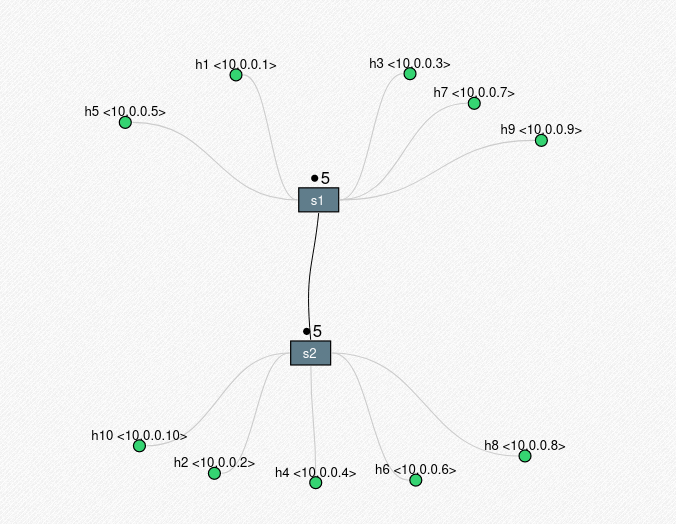
\includegraphics[width=0.9\linewidth]{images/mininet_topo.png}
    \caption{The resulting Dumbbell topology with the broker being h9 - the central node. The link between the central switch and the central host results in a congested network.}
    \label{fig:mininet-topo}
\end{figure}

Using the Python API provided, we created the network topology shown in Figure~\ref{fig:mininet-topo}.
The script takes several parameters to create the following three scenarios:

\begin{itemize}
    \item A synthetic scenario testing the limits of implementations.
    \item A realistic scenario based on a smart-home use-case.
    \item A realistic scenario based on a 3D printer farm.
\end{itemize}

The topology for all three scenarios remains the same - a minimum spanning tree of a typical IoT mesh network.
When designing this topology, we needed it to reflect various realistic IoT scenarios.
We can imagine this as a singular room in a home with all of its smart appliances being a cluster in the smart home or a cluster of 3D printers in a section of a farm in the 3D printer farm.
The critical feature of this topology is that many clusters are connected to a central broker that controls the topology, hence creating a dumbbell structure.
The full definition of this topology can be found in Appendix~\ref{appendix:topo}.
The variables that the script changes between scenarios and simulations are the link's \textit{bandwidth}, \textit{delay} and the rate of \textit{packet loss}.

The bandwidth of a link is the maximum rate of data transfer we can achieve.
In contrast to bandwidth in signal processing, we measure bandwidth in bits per second rather than hertz in computer networking.
The delay of a link specifies the latency of the link.
It is the time that a bit of data takes to travel across a link. 
We measure this in milliseconds.
Link delay corresponds to the geographical distance between the communicating parties; however, in the case of IoT, we can expect devices to be in local proximity.
Lastly, the packet loss rate shows the percentage of corrupted or dropped packets in transit.
Various protocols having to retransmit packets also adds to the delay of data transfer.
Importantly, we have only considered the typical circumstances of packet loss and have not included scenarios such as interference or packet loss attacks.

The bandwidth and delay numbers correspond, as closely as possible, to various link types in a network.
To do so, for the smart-home scenario, we have gathered data from the~\cite{ofcom_uk_2021} report on UK broadband speeds.
There were specific cases in which it was not possible to find this data in the report; hence it was augmented using a similar methodology in work conducted by~\cite{previdi_is-is_2019} and in the case of ZigBee, the work by~\citet{alena_fault_2011}.

\begin{table}[ht]
    \caption{The parameters chosen for each link simulation in Mininet in the smart home scenario. The types of links were chosen as the most commonly occurring ones in IoT use cases.}\label{tab:links:home}
    %\tt 
    \rowcolors{2}{}{gray!3}
    \begin{tabular}{@{}llll@{}}
        \toprule
        \textbf{Simulated Link Type} & \textbf{Link bandwidth (Mb/s)} & \textbf{Link delay (ms)} & \textbf{Packet loss rate (\%)} \\
        Wi-Fi                        & \texttt{30}                    & \texttt{10}              & \texttt{2}                     \\
        ZigBee                       & \texttt{0.25}                  & \texttt{5}               & \texttt{1}                     \\
        4G                           & \texttt{4}                     & \texttt{20}              & \texttt{1.5}                   \\
        3G                           & \texttt{1}                     & \texttt{40}              & \texttt{1.5}                   \\
        100Mb Ethernet               & \texttt{100}                   & \texttt{1}               & \texttt{0.2}                   \\
        \bottomrule
    \end{tabular}
\end{table}

Hence, we expect that the bandwidth and link delay numbers accurately represent a real-world scenario.
However, it was complicated to find exact estimates for packet loss rates, with most sources describing approximations for a stable connection~\citep{sdu_ictp-sdu_2013} and not precise measurements.
Hence, the data are best estimates, cross-validated through the different sources and are not exact values.

In the case of the smart home scenario, as presented in Table~\ref{tab:links:home}, we expect that our packet loss rates are accurate as these, as previously stated, do appear in the home broadband reports and other studies.
In the case of the 3D printer, as presented in Table~\ref{tab:links:3d} farm scenario, due to the number of machines and the interference these cause in a 3D printer farm, we modelled this scenario to have more packet loss.
We specifically chose this scenario to test the benefits that QUIC should receive in an environment with high packet loss.
However, we found it difficult to find exact data on packet loss percentages in smart factories or workshops; hence, we expect a margin of error on some of the values.

In general, we can assume that the packet loss rates will increase by some constant factor across all links.
Hence, we have also created a synthetic scenario with extreme packet loss as presented in Table~\ref{tab:links:synth}.
If the protocol performs well for an extreme scenario, we can expect it to also perform well for packet loss percentages up to that scenario.

\begin{table}[ht]
    \caption{The parameters chosen for each link simulation in Mininet in the 3D printer farm scenario. The data assumes a typical IoT setup where most devices are within local geographical proximity. That is, the devices are communicating with each other within the range of one factory or site, with only the central node communicating with some server.}\label{tab:links:3d}
    %\tt 
    \rowcolors{2}{}{gray!3}
    \begin{tabular}{@{}llll@{}}
        \toprule
        \textbf{Simulated Link Type} & \textbf{Link bandwidth (Mb/s)} & \textbf{Link delay (ms)} & \textbf{Packet loss rate (\%)} \\
        Wi-Fi                        & \texttt{30}                    & \texttt{10}              & \texttt{5}                     \\
        ZigBee                       & \texttt{0.25}                  & \texttt{5}               & \texttt{3}                     \\
        4G                           & \texttt{4}                     & \texttt{20}              & \texttt{2.5}                   \\
        3G                           & \texttt{1}                     & \texttt{40}              & \texttt{2.5}                   \\
        100Mb Ethernet               & \texttt{100}                   & \texttt{1}               & \texttt{0.5}                   \\
        \bottomrule
    \end{tabular}
\end{table}

\begin{table}[ht]
    \caption{The parameters chosen for each link simulation in Mininet in the synthetic scenario. Here we opt for extreme packet loss scenarios to test the boundaries of the protocols. We opted for 20 times the normal packet loss that the link can expect in each case. We have also tested this for higher values however all protocol implementations greatly suffered in performance beyond this.}\label{tab:links:synth}
    %\tt 
    \rowcolors{2}{}{gray!3}
    \begin{tabular}{@{}llll@{}}
        \toprule
        \textbf{Simulated Link Type} & \textbf{Link bandwidth (Mb/s)} & \textbf{Link delay (ms)} & \textbf{Packet loss rate (\%)} \\
        Wi-Fi                        & \texttt{30}                    & \texttt{10}              & \texttt{15}                     \\
        ZigBee                       & \texttt{0.25}                  & \texttt{5}               & \texttt{15}                     \\
        4G                           & \texttt{4}                     & \texttt{20}              & \texttt{20}                   \\
        3G                           & \texttt{1}                     & \texttt{40}              & \texttt{20}                   \\
        100Mb Ethernet               & \texttt{100}                   & \texttt{1}               & \texttt{4}                   \\
        \bottomrule
    \end{tabular}
\end{table}

We evaluate MQuicTT's performance using the presented topologies and respective simulation parameters in the following way.
Each protocol transmits 100 messages from a client to a broker for each data link.

During this, we measure the following:

\begin{itemize}
    \item The time taken for the underlying transport protocol to establish a connection.
    \item The time taken to transmit the message to the broker.
\end{itemize}

This is repeated several times to ensure that variance does not affect results.
This process is repeated for all three testing scenarios.

In general, MQTT allows for messages with a maximum size of approximately 260MB.
However, this is a huge message, and most publicly deployed brokers reject it, so we created a representative message for each use case.
Each topic in MQTT consists of a hierarchy of topic levels separated by a forward slash.
For example, in a smart home scenario, we may have a topic like $home/groundfloor/kitchen/temp$ to control the temperature in the kitchen via a smart thermostat.
A topic may also include a wildcard.
The topic string $home/groundfloor/+/temp$ includes a \textit{single-level} wildcard that will match an arbitrary string.
This would match the topic $home/groundfloor/lounge/temp$, but not match the topic $home/secondfloor/kitchen/temp$.
If a client wishes to subscribe to multiple topics with the same prefix, a \textit{multi-level} wildcard may be used.
For example, the topic $home/secondfloor/kitchen/\#$ can be used to subscribe to all topics with a prefix matching the string before the hash character.
Notably, brokers reserve topics for system messages starting with the \$ character.

The chosen topic and the transmitted message for each scenario can be found in Appendix~\ref{appendix:mqtt_message}.
The messages were devised based on an arbitrary command that may be issued to an IoT device present in the scenario.
For the synthetic scenario we opted to use a message that is considerably longer, to test the limits of each implementation.
This message simply consisted of a paylaod with a field replicated thousands of times.
It has ben omitted from the Appendix due to being too long.
\section{Connection time comparison} \label{sec:conn_time}

In this section of the analysis, we focus on connection time.
By connection time, we mean two things: the time it takes for the underlying transport protocol to establish a secure connection and the total time taken before MQTT sends its first data packet.

Connection time is essential in IoT devices as many do not connect while idling.
A device may opt not to be connected at all times to reduce energy consumption and computational power.
The device will then establish a connection and transmit data whenever required.
However, this means that some efficiency is lost if the connection has to be constantly re-established.
Hence, MQTT defines the period to keep the connection alive as the \textit{keep alive interval}.
In an MQTT/TCP implementation, the standard way to extend the keep alive interval is to periodically send a $ping$ packet, forcing the connection to remain open.
However, it has been shown that this method can lead to security vulnerabilities~\citep{vaccari_slowtt_2020,mileva_comprehensive_2021}.

We have talked previously about QUIC having a less complex handshake and hence being able to establish a secure connection quicker than TCP/TLS.
Hence, using QUIC in MQTT is a step closer to providing the needed efficiency while not having to use methods that may lead to vulnerabilities.

To measure the connection time we have began a communication via MQuicTT and the other MQTT implementations and captured it using $tcpdump$.
We have then extracted the time between the start of the QUIC or TCP communication and the completion of the handshake, as well as the time before MQTT sends its first data packet.
The results of this are shown in Figure TBA.

[Figure here]

[Discussion here]
\section{Data transmission comparison}

We next evaluate the time it took both implementations to transmit the aforementioned MQTT messages.
To do so, we have used the previously described methodology.
That is, we have transmitted the MQTT messages shown in~\ref{appendix:mqtt_message} for their respective scenario and have measured the total time taken for the transmission to occur.
We have repeated this and taken the average of the results to ensure that they are representative.

Based on the analysis of connection time and previous discussions, we hypothesise that:

\begin{itemize}
    \item \textbf{H1}: $MQuicTT$ performs on-par with $rumqtt$ in the IoT home scenario but does not present a significant difference.
    \item \textbf{H2}: $MQuicTT$ performs significantly better than $rumqtt$ in the printer farm scenario.
    \item \textbf{H3}: $MQuicTT$ can transmit all the messages on all data links in the synthetic scenario, whereas $rumqtt$ is not.
\end{itemize}

Figure~\ref{fig:comm_time} shows the results of this experiment.

We can see that the results support hypothesis \textbf{H1}.
That is,  $MQuicTT$ performs almost identically to $rumqtt$ across all data links for the IoT home scenario.
In fact, $MQuicTT$ actually performs marginally better than $rumqtt$ in this scenario with the transmission time of $MQuicTT$ being on average $2.02\%$ lower than that of $rumqtt$.
From this we can see that $MQuicTT$ presents no disadvantages in terms of transmission time even in network with low packet loss and congestion.
For new deployments it would be advantages to use $MQuicTT$, however, for existing ones, it may not be advisable to migrate deployments.

Hypothesis \textbf{H2} however is not supported.
The performance advantage in terms of transmission time for $MQuicTT$ in the printer farm scenario is almost identical to that of the smart home scenario.
On average, $MQuicTT$ transmits the data $2.36\%$ faster than $rumqtt$ and although this is an improvement, it is comparable to the improvement in the IoT home scenario.
Hence, the results draw a similar conclusion to that of the IoT home scenario.
It is still advantages to use $MQuicTT$ for new deployments.

The results of the printer farm scenario show that the presented use-case does not present a high enough packet loss percentage for $MQuicTT$ to have a significant advantage.
This can be verified by looking at the synthetic scenario, which validates hypothesis \textbf{H3}.
In the synthetic scenario only $MQuicTT$ managed to transmit the data on all data links and transmitted the data $13.8\%$ faster using ethernet.
Hence, in environments that may experience extreme data loss, $MQuicTT$ presents a clear advantage, however, finding such a scenario may be difficult.

Overall, $MQuicTT$ transmitted the data faster than $rumqtt$ across all scenarios and has shown to be more resilient against high packet loss.
It may however be ineffective overhead to migrate existing deployments to it due to the marginal benefits in low congestion environments.
\newpage
\section{Binary size experiment}

\subsection{Binary size experiment design} \label{sec:exp_bin}

This section describes how we have conducted further analysis on the binary size of the QUIC protocol that underlines $MQuicTT$.
The focus of this section is to see if the QUIC stack contributes a significant overhead to $MQuicTT$'s binary size and how we can reduce this overhead.
We expect that the QUIC stack will contribute to the majority of the size of $MQuicTT$ as MQTT itself is designed to have a low code size overhead.
Additionally, we have conducted a similar analysis for the TLS library used and expect that it also contributes a significant amount to the resulting binary size.
Hence, the first step of this part of the analysis will be to determine how much QUIC contributes to the binary size.

In order to get a breakdown of the binary we have used the $cargo-bloat$~\footnote{cargo-bloat - \url{https://lib.rs/crates/cargo-bloat}} utility.
This utility analyses the binary using custom ELF, DWARF and Mach-O parsers and disassembles the binary to look for references and links to anonymous data.
Doing so creates a map of the binary that shows where every byte has a label attached to it.

This utility provides the composition of a Rust binary. 
However, it is not perfect and results in some margin of error.
Unfortunately, this margin of error is also not easily measurable.
By comparing the total size of the binary as reported by $cargo-bloat$ to the size reported by the operating system, we have deduced that the total error margin is within $1\%$ with good precision.
This should mean that we can get a somewhat accurate error margin on the components. 
However, it is also possible that the internal calculations are inaccurate despite the overall size being accurate.

The next step in this stage will be analysing methods for trimming down the QUIC stack binary size.
Hence, in this stage, we shift our focus to the binary produced by $QuicSocket$.
To reduce the binary size, we opt to use the method established by~\citet{eggert_towards_2020} as recreating these steps may show a general framework for reducing binary sizes for hardware constrained devices.
Notably, our application already handles client and server code separately; the MQTT broker requires a different binary to the MQTT client.

Hence, the steps we take are as follows:

\begin{itemize}
    \item Compile the binary for a 32-bit target by setting the $target$ flag in cargo to $i686-unknown-linux-gnu$.
    \item Remove any error handling code beyond what is needed for the binary to compile.
    \item Remove any code that writes to standard output.
\end{itemize}

After every step, we record the difference in binary size made by the change using the same methodology.

Once this step is completed, we further analyse the size of $Quinn$ and $Rustls$ using a by-function binary size breakdown.
Using the $cargo-bloat$ utility, we can get a list of the contribution of each function to the binary size and then assign each function to its respective protocol feature.

\section{Binary size breakdown} \label{sec:binary_sizes}

We first look at an in-depth breakdown of the composition of the binary of the underlying QUIC implementation.
As previously established, hardware constrained devices do not have much space for firmware; hence, identifying sections of the QUIC stack that can be trimmed down or eliminated entirely is essential.
In order to get a breakdown of the binary we have used the $cargo-bloat$~\footnote{cargo-bloat - \url{https://lib.rs/crates/cargo-bloat}} utility.

[figure of results here]

[discussion of results here]

In order to reduce the binary size we opt to use the method established by~\citet{eggert_towards_2020} as recreating these steps may show a general framework for reducing binary sizes for hardware constrained devices.
Notably, our application already handles client and server code separately; the MQTT broker requires a different binary to the MQTT client.

Hence, the steps we have taken are as follows:

\begin{itemize}
    \item Compile the binary for a 32-bit target by setting the $target$ flag in cargo to $i686-unknown-linux-gnu$.
    \item Remove any error handling code beyond what is needed for the binary to compile.
    \item Remove any code that writes to standard output.
\end{itemize}

The resulting binary sizes after these steps can be found in Figure TBA.

[Figure here]

As we can see, after trimming down the binary, the TLS implementation stands out as the most considerable dependency.
While~\cite{eggert_towards_2020} attempts to address this by creating minimal cypher implementations used by TLS, we instead opt to discuss the possibility of a complete alternative to TLS, suitable for hardware constrained devices in Section~\ref{chap:TLS}.


\section{Summary}

When discussing the possibility of using a Rust QUIC implementation as the transport layer protocol for network firmware in IoT devices, we established that the QUIC implementation must perform at least as well as the baseline and have a binary size that can fit onto widely used IoT devices.

From the above analysis, we can conclude that $MQuicTT$ performs at least as well as the baseline TCP implementation of $rumqtt$.
When it comes to connection time, $MQuicTT$ performs marginally better, and when it comes to total transmission time, the implementations are on par.
Hence, this requirement is satisfied.

In terms of binary size, we have managed to reduce it to approximately $8Mb$ from a starting point of $9.1Mb$, a reduction of $12.1\%$.
We have also shown that the methods developed by~\citet{eggert_towards_2020} do translate to our implementation, implying that this could be a general methodology.
This size of binary would easily be installable on popular IoT devices such as the Raspberry Pi 3 Model B, Beagle Board or the Arduino Due.
However, this size of binary would not support industrially-wide used chips such as the esp32.
We have analysed the possible avenues of further reducing the binary size of $MQuicTT$ by addressing issues with the regex library and by analysing $Quinn$ and $Rustls$ by feature.
Hence, overall, we can say that we have achieved creating an implementation that can be used on a large number of IoT devices, but not on ones with stricter hardware constraints.
